\documentclass[11pt,a4paper]{article}
\usepackage[margin=2.5cm]{geometry}
\usepackage[T1]{fontenc}
\usepackage[utf8]{inputenc}
\usepackage{xcolor}
\usepackage{booktabs}
\usepackage{hyperref}
\usepackage{parskip}
\usepackage{pgfplots}
\usepackage{tikz}
\usepackage{array}
\usepackage{fancyhdr}
\usepackage{graphicx}
\pgfplotsset{compat=1.18}

% Brand colours
\definecolor{tregreen}{HTML}{1B3A2D}
\definecolor{tregold}{HTML}{C9A84C}
\definecolor{trelight}{HTML}{D8F3DC}
\definecolor{treblue}{HTML}{2E86AB}
\definecolor{trepurple}{HTML}{7B2D8B}
\definecolor{tregrey}{HTML}{6B7280}

\hypersetup{colorlinks=true,linkcolor=tregreen,urlcolor=treblue}

\pagestyle{fancy}
\fancyhf{}
\rhead{\small\color{tregrey}Treehouse Ghana — Instagram Report}
\lhead{\small\color{tregrey}\textbf{Confidential}}
\cfoot{\small\color{tregrey}\thepage}

\title{%
  \vspace{-1.5cm}
  {\color{tregreen}\Huge\bfseries Treehouse Ghana}\\[6pt]
  {\color{tregold}\large Instagram Performance Report}\\[4pt]
  {\normalsize Prepared 2026-05-31}
}
\author{}
\date{}

\begin{document}
\maketitle
\thispagestyle{fancy}

% ─── KEY METRICS BOX ──────────────────────────────────────────────────────────
\noindent
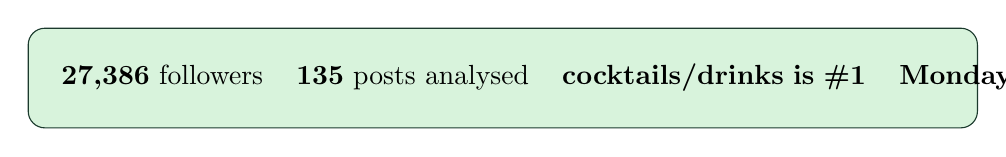
\begin{tikzpicture}
\node[draw=tregreen,fill=trelight,rounded corners=6pt,inner sep=12pt,text width=\linewidth-26pt]{%
  \begin{tabular}{@{}llll@{}}
    \textbf{27,386} followers &
    \textbf{135} posts analysed &
    \textbf{cocktails/drinks is \#1} &
    \textbf{Monday best day}\\
  \end{tabular}
};
\end{tikzpicture}
\vspace{8pt}

% ─── EXECUTIVE SUMMARY ────────────────────────────────────────────────────────
\section*{\color{tregreen}Executive Summary}

Treehouse Ghana has 27,386 followers.
This report analyses 135 posts and short videos published over the past 18 months.
Key findings:

\begin{enumerate}
  \item \textbf{Cocktails and drinks is the strongest content category}, followed by cocktails and drinks, events and live music, ambience. Do more of what already works.
  \item \textbf{Short videos attract more engagement than feed posts on average} and reach beyond existing followers; expanding video is a clear opportunity.
  \item \textbf{Monday is the best day to post}, with the highest average engagement.
  \item \textbf{Audience comments are warm and specific} — praise for the food and questions about events and booking. Replying quickly turns a comment into a customer.
  \item \textbf{Posts that feature the business (customer posts, collaborations) draw strong engagement} — reshare them and lean into that social proof.
\end{enumerate}

% ─── CONTENT PERFORMANCE ──────────────────────────────────────────────────────
\section*{\color{tregreen}What Content Performs Best}

The chart below ranks each content type by average engagement score.
A higher score means more likes, comments and video plays combined.

\vspace{8pt}
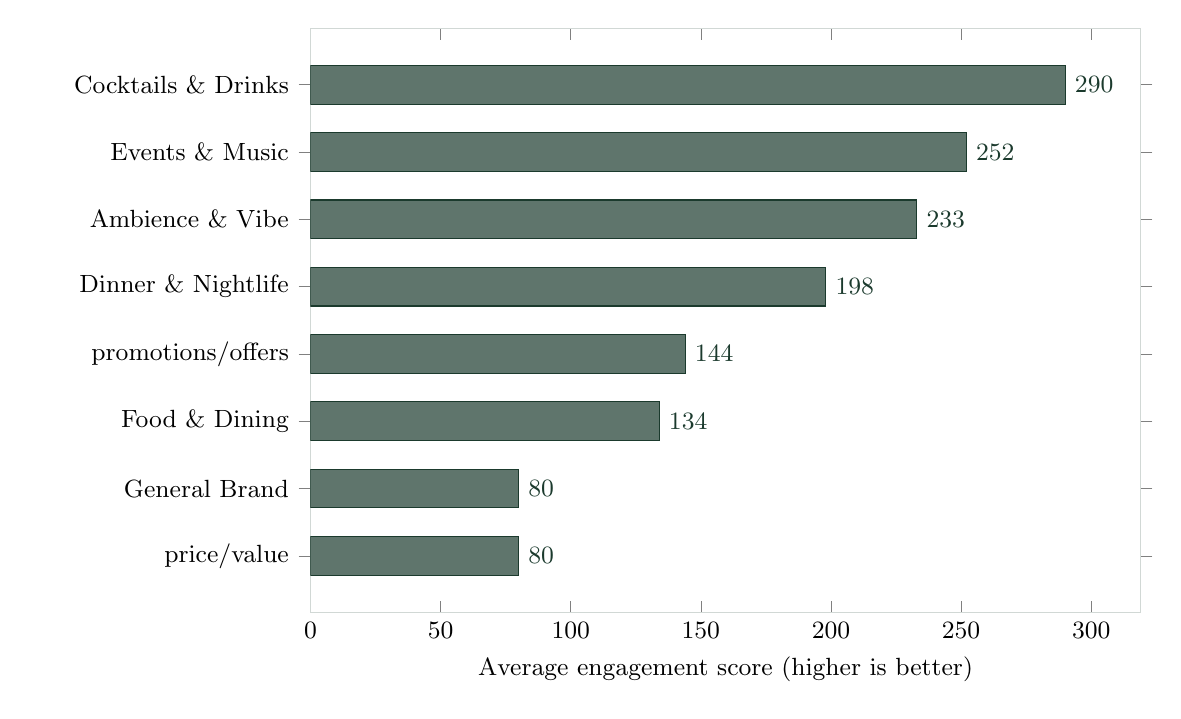
\begin{tikzpicture}
\begin{axis}[
  xbar,
  width=\linewidth,
  height=9cm,
  bar width=14pt,
  xlabel={\small Average engagement score (higher is better)},
  symbolic y coords={price/value,General Brand,Food \& Dining,promotions/offers,Dinner \& Nightlife,Ambience \& Vibe,Events \& Music,Cocktails \& Drinks},
  ytick=data,
  xmin=0,
  scaled x ticks=false,
  xticklabel style={/pgf/number format/.cd,fixed,precision=0,1000 sep={,}},
  nodes near coords={\pgfmathprintnumber[fixed,precision=0,1000 sep={,}]{\pgfplotspointmeta}},
  nodes near coords align={horizontal},
  every node near coord/.style={font=\small,color=tregreen},
  tick label style={font=\small},
  label style={font=\small},
  y tick label style={align=right,text width=3.2cm},
  draw=tregreen!20,
  fill=tregreen!60,
  enlarge y limits=0.12,
]
\addplot[fill=tregreen!70,draw=tregreen] coordinates {
  (80,{price/value})
  (80,{General Brand})
  (134,{Food \& Dining})
  (144,{promotions/offers})
  (198,{Dinner \& Nightlife})
  (233,{Ambience \& Vibe})
  (252,{Events \& Music})
  (290,{Cocktails \& Drinks})
};
\end{axis}
\end{tikzpicture}

% ─── SHORT VIDEOS ─────────────────────────────────────────────────────────────
\section*{\color{tregreen}Short Videos vs Feed Posts}

\begin{center}
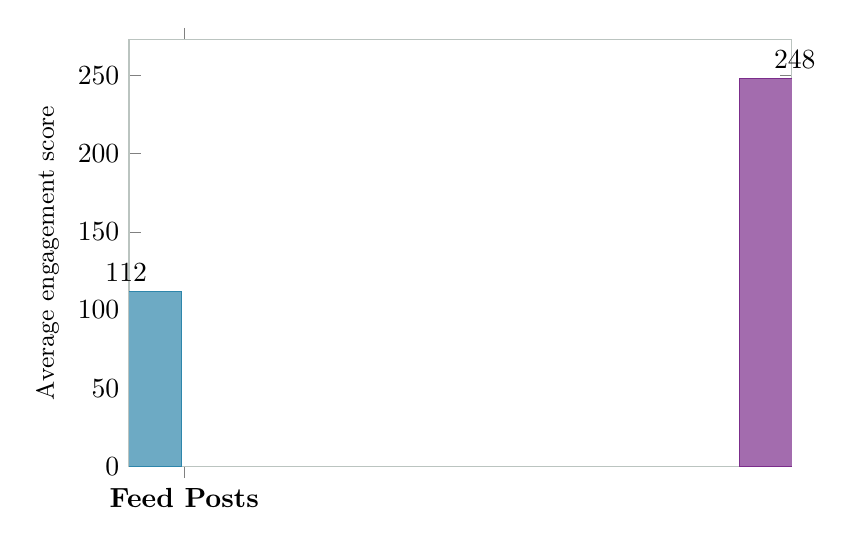
\begin{tikzpicture}
\begin{axis}[
  ybar,
  width=10cm,
  height=7cm,
  bar width=40pt,
  ylabel={\small Average engagement score},
  symbolic x coords={Feed Posts, Short Videos (Reels)},
  xtick=data,
  ymin=0,
  scaled y ticks=false,
  yticklabel style={/pgf/number format/.cd,fixed,precision=0,1000 sep={,}},
  nodes near coords={\pgfmathprintnumber[fixed,precision=0,1000 sep={,}]{\pgfplotspointmeta}},
  nodes near coords align={vertical},
  tick label style={font=\normalsize\bfseries},
  axis line style={draw=tregreen!30},
]
\addplot[fill=treblue!70,draw=treblue] coordinates {(Feed Posts,112)};
\addplot[fill=trepurple!70,draw=trepurple] coordinates {(Short Videos (Reels),248)};
\end{axis}
\end{tikzpicture}
\end{center}

\textbf{Short videos attract more engagement than feed posts on average} and reach beyond existing followers; expanding video is a clear opportunity.
Short videos reach people who do not yet follow the account through Instagram's discovery algorithm, which is why they are worth using.  Measure their reach in your native Instagram Insights, which this public analysis cannot see.

% ─── BEST DAYS ────────────────────────────────────────────────────────────────
\section*{\color{tregreen}Best Days to Post}

\begin{center}
\begin{tabular}{lrc}
\toprule
\textbf{Day} & \textbf{Avg Engagement} & \textbf{Recommendation} \\
\midrule
Monday & 199 \\
Tuesday & 180 \\
Friday & 148 \\
Thursday & 141 \\
Sunday & 121 \\
Saturday & 104 \\
Wednesday & 95 \\
\bottomrule
\end{tabular}
\end{center}

% ─── COMMENT INTELLIGENCE ─────────────────────────────────────────────────────
\section*{\color{tregreen}What Your Audience is Saying}

We classified \textbf{106 comments} from your top-performing posts.
Every location question, booking request and menu enquiry is a warm lead.

\begin{center}
\begin{tabular}{lrr}
\toprule
\textbf{Comment type} & \textbf{Count} & \textbf{Share} \\
\midrule
General reactions & 86 & 81.1\% \\
Positive praise & 8 & 7.5\% \\
Atmosphere praise & 5 & 4.7\% \\
Location questions & 5 & 4.7\% \\
Event questions & 3 & 2.8\% \\
date-night/romantic ambience & 3 & 2.8\% \\
Menu curiosity & 2 & 1.9\% \\
Service feedback & 1 & 0.9\% \\
\bottomrule
\end{tabular}
\end{center}

\textbf{Actionable:} Reply to every booking request, location question and event enquiry within 30 minutes.
Include your WhatsApp number in every post that mentions dining or bookings.

% ─── STRATEGY SCENARIOS ───────────────────────────────────────────────────────
\section*{\color{tregreen}Three Scenarios for Growth}

The table below shows expected 12-week engagement totals under three approaches.
These are projections based on 10,000 simulations of historical performance.

\begin{center}
\begin{tabular}{lrcc}
\toprule
\textbf{Approach} & \textbf{Expected Total} & \textbf{Likely Range} & \textbf{vs Today} \\
\midrule
Current approach & 6,773 & 3696–10378 & 0\% \\
Improved mix & 8,836 & 5360–12787 & 30.5\% \\
Video focus & 12,004 & 7877–16451 & 77.2\% \\
\bottomrule
\end{tabular}
\end{center}

% ─── RECOMMENDATIONS ──────────────────────────────────────────────────────────
\section*{\color{tregreen}Recommended Actions}

\subsection*{This week}
\begin{enumerate}
  \item Reply to every commercial comment (booking, location, menu, event questions).
  \item Add your WhatsApp number and reservation link to your Instagram bio.
  \item Create a \textquotedblleft Book a Table\textquotedblright{} Highlight with address, hours and contact details.
\end{enumerate}

\subsection*{This month}
\begin{enumerate}
  \setcounter{enumi}{3}
  \item Film three short videos: food being served, cocktails being poured, venue atmosphere.
  \item Post your next event with full date, time, lineup and booking instructions.
  \item Reshare two positive customer mentions and add your booking CTA.
\end{enumerate}

\subsection*{This quarter}
\begin{enumerate}
  \setcounter{enumi}{6}
  \item Shift your content calendar toward cocktails, events and ambience (your top categories).
  \item Set a 30-minute response-time target for Instagram comments during business hours.
  \item Re-run this analysis in 90 days to measure progress.
\end{enumerate}

\section*{\color{tregreen}How to Read This Report}

All figures are based on \textbf{public} Instagram data only.
Private metrics — reach, impressions, saves, profile visits, link clicks — are not included
and remain visible only in your native Instagram Insights dashboard.
The engagement score used throughout is: \textit{likes + (comments $\times$ 5) + (video plays $\div$ 100)}.
A higher score indicates a post attracted more visible audience interaction.

\vfill
\begin{center}
{\small\color{tregrey}Generated automatically from the Treehouse Ghana Instagram analysis pipeline.
Source code and data: \url{https://github.com/bernardashiley/treehouse-ghana-ig-insights}}
\end{center}

\end{document}
